\chapter{Data analysis}  \label{ch:data-analysis}

The MD evaluation of the GK integral, Eq.~\eqref{eq:GK}, usually proceeds in two steps. One first evaluates the integrand as a running average of the time-lagged current products, $\langle J^i(\tau)J^j(0)\rangle \sim \frac{1}{\mathcal{T}-\tau} \int_0^{\mathcal{T}-\tau} J^i(t+\tau)J^j(t)dt$, where $\mathcal{T}$ is the length of the MD trajectory.
The matrix defined in Eq.~\eqref{eq:L_def} is then estimated as a function of the upper limit of integration:  $L^{ij}(\mathcal{T})\propto \frac{\rOmega}{k_B} \int_0^\mathcal{T} \langle J^i(\tau)J^j(0)\rangle \,d\tau$. One then recovers, via Eq.~\eqref{eq:multi_kappa}, an estimate for the thermal conductivity depending on $\mathcal{T}$:
$\kappa(\mathcal{T})\propto \frac{1}{(L^{-1}(\mathcal{T}))^{\smallone\smallone}}$.
This function is usually very noisy: in fact, at times greater than the correlation time between $J^i$ and $J^j$, the correlation function $\langle J^i(\tau)J^j(0)\rangle$ approaches zero, hence $L^{ij}(\mathcal{T})$ starts integrating noise and behaves like the distance traveled by a random walk, whose variance grows linearly with the upper integration limit.
The evaluation of transport coefficients thus requires averaging over multiple trajectories (possibly multiple segments of a same long trajectory) and estimating the resulting uncertainty as a function of both the length of each trajectory and the upper limit of integration. This is a cumbersome task that often leads to a poor estimate of the statistical and systematic errors on the computed conductivity. All the more so when the signal is inherently oscillatory, due to the existence of high-frequency features in the power spectrum of the energy flux, possibly due to intramolecular oscillations that meddle with the noise. Some authors try to overcome these problems by either fitting the autocorrelation function or the GK integral with a multi-exponential function \citep{Schelling2002,Zhang2015}, or by extrapolating the power spectrum of the energy flux to the zero-frequency limit \citep{Volz2000}. Others have attempted an error analysis of the MD estimate of the GK integral, based on either heuristic or rigorous arguments \citep{Jones2012,Wang_gk2017,Oliveira2017}, but they all require an estimate of an optimal value for the upper limit of integration, which determines a bias in the estimate, and which is in general difficult to obtain. Different classes of systems require different approaches to error analysis, but it is widely believed that all of them always require so long simulation times as to be unaffordable with accurate but expensive AIMD techniques \citep{Carbogno:2017gc}. In order to solve this problem, \cite{Ercole2017} considered it in the light of the statistical theory of stationary time series.


\section{Solids and one-component fluids} \label{sec:univariate}
In practice, MD gives access to a discrete sample of the flux process (a \emph{time series}), $J_n = J(n \epsilon)$, $0 \leq n \leq N-1$, where $\epsilon$ is the sampling period of the flux and $N$ the length of the time series, that we assume to be even. As was shown in Sec.~\ref{sec:Einstein}, the Wiener-Khintchine theorem allows one to express the heat conductivity in terms of the zero-frequency value of the power spectrum of the energy-flux (see Eqs.~(\ref{eq:Wiener-Khintchine}-\ref{eq:GK-S0})):
\begin{equation}
\kappa = \frac{\rOmega}{2k_B T^2} S (\omega=0). \label{eq:kappa-S0}
\end{equation}
Let us define the discrete Fourier transform of the flux time series as:
\begin{equation}
  \tilde{J}_{k}=\sum_{n=0}^{N-1} \mathrm{e}^{ 2\pi i\frac{kn}{N}} J_n, \label{eq:Jk}
\end{equation}
for $0 \leq k \leq N-1$.\footnote{Here, the convention for the sign in the exponential of the time-to-frequency Fourier transform is opposite to what adopted in \citep{Ercole2017} and in most of the signal analysis literature, in order to comply with the convention for the space-time Fourier transforms usually adopted in the Physics literature and in Eqs.~\eqref{eq:kontinuity} and \eqref{eq:Fourier-continuity}.} The \emph{sample spectrum} $\hat S_k$, aka \emph{periodogram}, is defined as
\begin{equation}
\hat{S}_{k}=\frac{\epsilon}{N} \left |\tilde{J}_{k} \right |^2, \label{eq:periodogram-def}
\end{equation}
and, for large $N$, it is an unbiased estimator of the power spectrum of the process, as defined in Eq.~\eqref{eq:Wiener-Khintchine}, evaluated at $\omega_k=2\pi\frac{k}{N\epsilon}$, namely: $\langle \hat S_k \rangle = S(\omega_k)$. The reality of the $\hat J$'s implies that $\tilde J_k=\tilde J^*_{N-k}$ and $\hat S_k=\hat S_{N-k}$, so that periodograms are usually reported for $0\leq k\leq \frac{N}{2}$ and their Fourier transforms evaluated as discrete cosine transforms.

The space autocorrelations of conserved currents are usually short-ranged. Therefore, in the thermodynamic limit the corresponding fluxes can be seen as sums of (almost) independent identically distributed stochastic variables, so that, according to the central-limit theorem, their equilibrium distribution is Gaussian. A slight generalization of this argument allows us to conclude that any conserved-flux process is Gaussian as well. The flux time series is in fact a multivariate stochastic variable that, in the thermodynamic limit, results from the sum of (almost) independent variables, thus tending to a multivariate normal deviate. This implies that at equilibrium the real and imaginary parts of the $\tilde J_k$'s defined in Eqs.~\eqref{eq:Jk} are zero-mean normal deviates that, in the large-$N$ limit, are uncorrelated among themselves and have variances proportional to the power spectrum evaluated at $\omega_k$. For $k=0$ or $k=\frac{N}{2}$, $\tilde J_k$ is real and $\sim \mathcal{N}\left (0, \frac{N}{\epsilon}S(\omega_k) \right )$; for $k\notin\left\{ 0,\frac{N}{2}\right\}$, $\mathfrak{Re}\tilde{J}_k$ and $\mathfrak{Im}\tilde{J}_k$ are independent and both  $\sim \mathcal{N}\left (0, \frac{N}{2 \epsilon}S(\omega_k) \right )$, where $\mathcal{N} (\mu,\sigma^2)$ indicates a normal deviate with mean $\mu$ and variance $\sigma^2$. We conclude that in the large-$N$ limit the sample spectrum of the heat-flux time series reads:
\begin{equation}
\hat{S}_{k} = S \left(\omega_k\right) {\xi}_{k}, \label{eq:periodogram-distribution}
\end{equation}
where the $ {\xi}$'s are independent random variables distributed as a $\chi_1^2$ variate for $k=0$ or $k=\frac{N}{2}$ and as one half a $\chi_2^2$ variate, otherwise. Here and in the following $\chi^2_\nu$ indicates the chi-square distribution with $\nu$ degrees of freedom. For the sake of simplicity, we make as though all the ${\xi}$'s were identically distributed, $\xi_k \sim \frac{1}{2} \chi_2^2$ for all values of $k$, thus making an error of order $\mathcal{O}(1/N)$, which vanishes in the long-time limit that is being assumed throughout this section.

In many cases of practical interest, multiple time series are available to estimate the power spectrum of a same process, $\{{^p\!}J_n\}$, $p=1, \cdots \ell$. For instance, in equilibrium MD a same trajectory delivers one independent time series per Cartesian component of the heat flux, all of which are obviously equivalent in isotropic systems. In these cases it is expedient to define a mean sample spectrum by averaging over the $\ell$ different realizations,
\begin{equation}
    \begin{aligned}
      {^{\ell\!}\hat{S}}_{k}& = \frac{\epsilon}{\ell N} \sum_{p=1}^{\ell}  \left |{^p\!}{\tilde J}_{k} \right |^2 \\
      & = S \left(\omega_k\right) {^{\ell\!}{\xi}_{k}},
    \end{aligned} \label{eq:mean-periodogram}
\end{equation}
where the ${^{\ell\!}\xi}$'s are $\chi_{2\ell}^2$ variates, divided by the number of degrees of freedom: $^{\ell\!}\xi_{k}\sim\frac{1}{2\ell}\chi_{2\ell}^{2}$ $\bigl (\text{for } k \notin \{ 0,\frac{N}{2} \}\bigr )$.

\begin{figure}
\centering
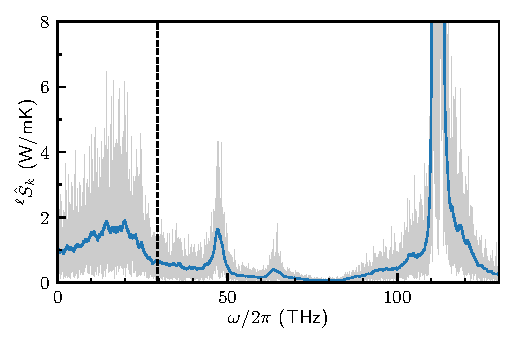
\includegraphics[width=8cm]{chapters/chapter5/figures/handbook_water_psd.pdf}
\caption{Periodogram of a classical flexible model of water obtained from a $100\un{ps}$ MD trajectory. Grey: periodogram obtained directly from Eq.~\eqref{eq:mean-periodogram}, with $\ell=3$. Blue: periodogram filtered with a moving average window of width $1\un{THz}$, useful to reveal the main features of the spectrum (see text). The vertical dashed line delimits the low-frequency region used in the subsequent cepstral analysis.}  \label{fig:water-periodogram}
\end{figure}

Eqs.~\eqref{eq:periodogram-distribution}) and \eqref{eq:mean-periodogram} show that ${^{\ell\!}}{\hat S_0}$ is an unbiased estimator of the zero-frequency value of the power spectrum, $\langle {^{\ell\!}}{\hat S_0} \rangle = S(0)$, and through Eq.~\eqref{eq:kappa-S0}, of the transport coefficients we are after. However, this estimator is not consistent, \emph{i.e.} its variance does not vanish in the large-$N$ limit. This is so because a longer time series increases the number of discrete frequencies at which the power spectrum is sampled, rather than its accuracy at any one of them.

Fig.~\ref{fig:water-periodogram} displays the periodogram of water at ambient conditions, obtained from a $100\un{ps}$ classical MD trajectory, showing the extremely noisy behavior of the periodogram as an estimator of the spectrum. Averaging over the values of the periodogram within a frequency window of given width \citep{MovingAverage} would consistently reduce the statistical noise, but the multiplicative nature of the latter in Eq.~\eqref{eq:periodogram-distribution} makes it difficult to disentangle the noise from the signal and may introduce a bias. In order to cope with this problem, we had better transform the multiplicative noise into an additive one by defining the log-periodogram, $^{{\ell\!}}\hat{L}_{k}$, as:
\begin{equation}
  \begin{aligned}
    ^{{\ell\!}}\hat{L}_{k} &= \log \left (^{\ell\!}\hat{S}_{k} \right ) \\
    &= \log\left(S(\omega_k) \right) + \log\left( ^{\ell\!}{\xi}_k\right ) \\
    &= \log\left(S(\omega_k) \right) + {^{\ell\!}\rLambda} + {^{\ell\!}{\lambda}}_{k},
  \end{aligned} \label{eq:log-PSD}
\end{equation}
where $^{\ell\!}{\lambda}_k = \log\left( {^{\ell\!}{\xi}}_k\right) - {^\ell{\rLambda}}$
are zero-mean identically distributed independent stochastic variables, ${^{\ell\!}\rLambda} = \left\langle \log\left( {^{\ell\!}{\xi}}\right ) \right\rangle = \psi(\ell)-\log(\ell)$, and $\psi(z)$ and is the digamma function \citep{PolyGamma}. The variance of the $^{\ell\!}\lambda$ variables is $\sigma_{\ell}^{2} =\psi'(\ell)$, where $\psi'(z)$ is the tri-gamma function \citep{PolyGamma}.

Whenever the number of (inverse) Fourier components of the logarithm of the power spectrum is much smaller than the length of the time series, applying a low-pass filter to Eq.~\eqref{eq:log-PSD} would result in a reduction of the power of the noise, without affecting the signal. In order to exploit this idea, we define the ``\emph{cepstrum}'' of the time series as the inverse Fourier transform of its sample log-spectrum \citep{Childers1977}:
\begin{equation}
  ^{\ell\!} \hat C_{n} = \frac{1}{N}\sum_{k=0}^{N-1} {^{\ell\!} \hat L_{k}} \mathrm{e}^{-2\pi i\frac{kn}{N}}. \label{eq:sample-cepstrum}
\end{equation}
A generalized central-limit theorem for Fourier transforms of stationary time series ensures that, in the large-$N$ limit, these coefficients are a set of independent (almost) identically distributed zero-mean normal deviates \citep{Anderson1994,Peligrad2010}. It follows that:
\begin{equation}
  \begin{aligned}
    ^{\ell\!} \hat  C_{n} &= \lambda_{\ell} \delta_{n0} + C_{n} +  {^{{\ell\!}}{\mu}}_{n}, \\
    C_{n} &= \frac{1}{N}\sum_{k=0}^{N-1} \log\bigl (S(\omega_k) \bigr ) \mathrm{e}^{-2\pi i\frac{kn}{N}},
  \end{aligned} \label{eq:cepstrogram}
\end{equation}
where $^{{\ell\!}}{\mu}_{n}$ are independent zero-mean \emph{normal} deviates with variances $\left\langle {^{{\ell\!}}{\mu}_{n}^2}  \right\rangle$ $=\frac{1}{N}\sigma_\ell$ for $n\notin\left\{ 0,\frac{N}{2}\right\}$ and $\left\langle ^{{\ell\!}}{\mu}_{n}^{2}\right\rangle =\frac{2}{N}\sigma_{\ell}^{2}$
otherwise.
Fig.~\ref{fig:water-cepstrum} displays the cepstral coefficients of the low-frequency region of the spectrum of water (marked in Fig.~\ref{fig:water-periodogram}), showing that only the first few coefficients are substantially different from zero.

\begin{figure}
\centering
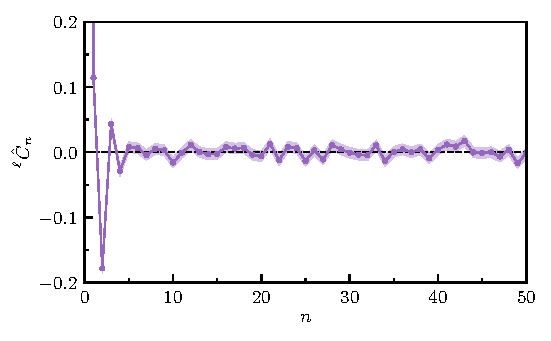
\includegraphics[width=8cm]{chapters/chapter5/figures/handbook_water_cepstrum.pdf}
\caption{Cepstral coefficients of water computed analyzing the low-frequency region of the periodogram (see Fig.~\ref{fig:water-periodogram}), defined in Eq.~\eqref{eq:sample-cepstrum}. }  \label{fig:water-cepstrum}
\end{figure}

Let us indicate by $P^*$ the smallest integer such that $C_n \approx 0$ for $P^* \le n \le N-P^*$. By limiting the Fourier transform of the sample cepstrum, Eq.~\eqref{eq:sample-cepstrum}, to $P^*$ coefficients, we obtain an efficient estimator of the zero-frequency component of the log-spectrum as:
\begin{equation}
  \begin{aligned}
    ^{{\ell\!}}\hat{L}_{0}^{*} & = {^{\ell\!}\hat{C}}_{0}+2\sum_{n=1}^{P^{*}-1}{^{{\ell\!}}\hat{C}}_{n} \\
    & = {^{\ell\!}\rLambda} + \log(S_0) + {^{{\ell\!}} {\mu}_{0}}+ 2 \sum_{n=1}^{P^*-1} {^{\ell\!} {\mu}_{n}}.
  \end{aligned} \label{eq:L0*}
\end{equation}
Inspection of Eq.~\eqref{eq:L0*} shows that $^{\ell\!}\hat{L}_{0}^{*}$ is a normal estimator whose expectation and variance are:
\begin{align}
	\langle {^{{\ell\!}}\hat{L}_{0}^{*}}\rangle &= \log(S_{0}) + {^{\ell\!}\rLambda}, \label{eq:L*} \\
	\sigma_\ell^{*}(P^{*},N)^{2} &=\sigma_{\ell}^{2}\frac{4P^{*}-2}{N}. \label{eq:sigma*}
\end{align}
Using Eq.~\eqref{eq:kappa-S0}, we see that the logarithm of the conductivity can be estimated from the cepstral coefficients of the flux time series through Eqs.~(\ref{eq:L0*}-\ref{eq:sigma*}), and that the resulting estimator is always normal with a variance that depends on the specifc system \emph{only} through the number of these coefficients, $P^*$. Notice that the absolute error on the logarithm of the conductivity directly and nicely yields the relative error on the conductivity itself.

The efficacy of this approach obviously depends on our ability to estimate the number of coefficients necessary to keep the bias introduced by the truncation to a value smaller than the statistical error, while maintaining the magnitude of the latter at a prescribed acceptable level. \cite{Ercole2017} proposed to estimate $P^*$ using the Akaike's information criterion (\cite{Akaike1974}), but other more advanced \emph{model selection} approaches \citep{Claeskens2008} may be more effective. This method consists in choosing $P^*$ as the one that minimizes the function:
\begin{equation}
\mathrm{AIC}(P)=\frac{N}{\sigma_\ell^{2}}\sum_{n=P}^\frac{N}{2} \hat{C}_{n}^{2}+2P. \label{eq:AIC-P}
\end{equation}
In Fig.~\ref{fig:water-filtered-psd} we report the low-frequency region of the spectrum of water obtained by limiting the number of cepstral coefficients to $P^*$:
\begin{equation}
^\ell\hat{S}_k^* = \exp\left[ 2\sum_{n=1}^{P^*-1} {}^\ell\hat{C}_n \mathrm{e}^{2\pi i \frac{k n}{N}} + {}^\ell\hat{C}_0 - {}^\ell\rLambda\right], \label{eq:filtered-psd}
\end{equation}
thus showing the filtering effect of this choice.
Finally, Fig.~\ref{fig:water-fkappa-Pstar} shows the value of thermal conductivity of water obtained through Eqs.~(\ref{eq:L0*}-\ref{eq:sigma*}).

\begin{figure}
    \centering
    \begin{center}
        \subfigure[\label{fig:water-filtered-psd}]{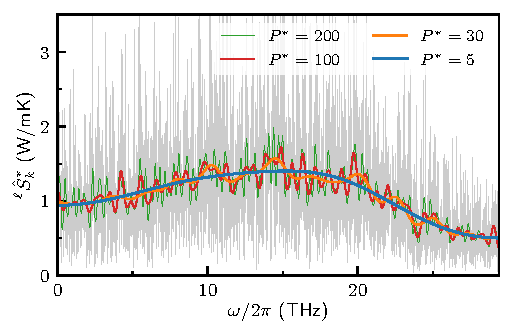
\includegraphics[width=8cm]{chapters/chapter5/figures/handbook_water_filtered_psd.pdf}}
        \subfigure[\label{fig:water-fkappa-Pstar}]{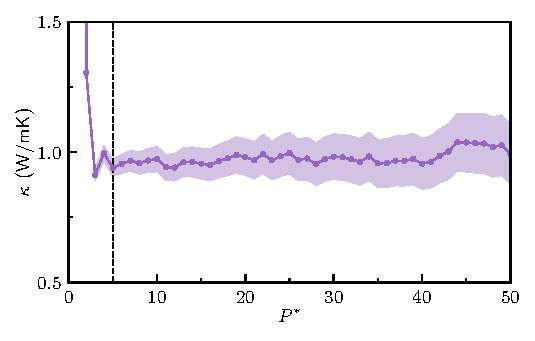
\includegraphics[width=8cm]{chapters/chapter5/figures/handbook_water_kappa_Pstar.pdf}}
    \end{center}
    \caption{
    (a) Filtered low-frequency region of the power spectrum of water obtained by limiting the number of cepstral coefficients to various values of $P^*$, Eq.~\eqref{eq:filtered-psd}. $P^*=7$ is the cutoff value suggested by the Akaike's information criterion, Eq.~\eqref{eq:AIC-P}. Grey: the unfiltered periodogram obtained from Eq.~\eqref{eq:periodogram-def}.
    (b) Thermal conductivity of water estimated from Eqs.~(\ref{eq:L0*}-\ref{eq:sigma*}) as a function of the cutoff, $P^*$. The colored bands indicate one standard deviation as estimated from theory. The vertical dashed line indicates the value suggested by the Akaike's information criterion, Eq.~\eqref{eq:AIC-P}.
    }
\end{figure}


\section{Multi-component fluids}
In Sec.~\ref{sec:multi-component} we have seen that in a fluid made of $Q$ atomic species there are in general $Q$ macroscopic fluxes interacting with each other through Onsager's phenomenological equations, Eq.~\eqref{eq:onsager}, not counting the different Cartesian components that do not interact amongst themselves because of space isotropy. A MD simulation thus samples $Q$ stochastic processes, one for each interacting flux, that we suppose to be stationary. These processes can be thought of as different components of a same multivariate process \citep{Bertossa2018}. As in Sec.~\ref{sec:univariate}, for the sake of generality we suppose to have $\ell$ independent samples of such a process, described by a multivariate time series of length $N$: $\{ ^{p\!}{J}^i_n \}$; $p=1,\dots \ell$; $i=1,\dots Q$; $n=0,\dots N-1$. Stationarity implies that $\langle {J}^i_n\rangle $ does not depend on $n$ and that $\langle {J}^i_n {J}^j_m \rangle$ only depends on $n-m$. We will further assume that $\langle {J}^i_n\rangle =0 $ and that $\langle {J}^i_n {J}^j_0 \rangle$ is an even function of $n$, which is the case when ${J}^i$ and ${J}^j$ have the same signature under time-reversal. By combining Eq.~\eqref{eq:multi_kappa} with Eq.~\eqref{eq:GK-S0}, we see that in order to evaluate the thermal conductivity in the multi-component case we need an efficient estimator for $\left ( S^{-1}_0\right )^{11}$, where $S^{kl}_0=S^{kl}(\omega=0)$ is the zero-frequency cross-spectrum of the relevant fluxes, ordered in  such a way that the energy one is the first.

Similarly to the one-component case, we define a mean sample cross-spectrum (or \emph{cross-periodogram}) as
\begin{equation}
 ^{(\ell Q)\!}\hat{S}_k^{ij} = \frac{1}{\ell} \sum_{p=1}^{\ell} \frac{\epsilon}{N} \left({}^{p\!}\tilde{J}_k^i\right)^* {}^{p\!}\tilde{J}_k^j .
\end{equation}
By discretizing Eq.~\eqref{eq:Sij(omega)} we see that $^{(\ell Q)\!}\hat{S}_k^{ij}$ is an unbiased estimator of the cross-spectrum, $\left \langle {}^{(\ell Q)\!}\hat{S}_k^{ij} \right \rangle = S^{ij}\left (\omega_k= \frac{2\pi k }{N\epsilon}\right )$. As it was the case for univariate processes, in the large-$N$ limit the real and imaginary parts of $\tilde J^i_k$ are normal deviates that are uncorrelated for $k\ne k'$. We conclude that the cross-periodogram is a random matrix distributed as a complex Wishart deviate \citep{Goodman1963a,Goodman1963b}:
\begin{equation}
  {}^{(\ell Q)\!}\hat{S}_k \sim \mathcal{CW}_Q \left(S(\omega_k), \ell\right). \label{eq:ComplexWishart}
\end{equation}
The notation $\mathcal{CW}_Q \left(S, \ell \right)$ in Eq.~\eqref{eq:ComplexWishart} indicates the distribution of the $Q\times Q$ Hermitian matrix
${}^{(\ell Q)\!}\hat{S}^{ij} = \frac{1}{\ell}\sum_{p=1}^\ell  {}^{p\!}{X}^i \, {}^{p\!}{X}^{j*}$,
where $\{ {}^{p\!}{X}^i \}$ ($p=1,\cdots\ell$, $i=1, \cdots Q$) are $\ell$ samples of an $Q$-dimensional zero-mean normal variate whose covariance is $S^{ij} = \langle X^i X^{j*} \rangle $.

Similarly to the real case, a Bartlett decomposition \citep{kshirsagar1959} holds for complex Wishart matrices \citep{Nagar2011}, reading:
\begin{equation}
{}^{(\ell Q)\!}\hat{S} = \frac{1}{\ell} \mathcal{S} R R^\top \mathcal{S}^{\dagger},  \label{eq:S_cholesky}
\end{equation}
where ``$\top$'' and ``$\dagger$'' indicate the transpose and the adjoint of a real and complex matrix, respectively; $\mathcal{S}$ is the Cholesky factor of the covariance matrix, $S= \mathcal{S} \mathcal{S}^{\dagger}$, and $R$ is a real lower triangular random matrix of the form
\begin{equation}
 R =
 \begin{pmatrix}
 c_1 & 0 & 0 & \cdots & 0\\
 n_{21} &  c_2 &0 & \cdots& 0 \\
 n_{31} &  n_{32} &  c_3 & \cdots & 0\\
\vdots & \vdots & \vdots &\ddots & \vdots \\
 n_{\smallQ1} & n_{\smallQ2} & n_{\smallQ3} &\cdots & c_\smallQ
 \end{pmatrix},
\end{equation}
where $c^2_i \sim \chi^2_{2(\ell-i+1)}$ and $ n_{ij}\sim \mathcal{N}(0,1)$. We stress that $R$ is independent of the specific covariance matrix, and only depends upon $\ell$ and $Q$. In particular it is independent of the ordering of the fluxes $J^i$. By expressing the $QQ$ matrix element of the inverse of $^{(\ell Q)}\hat{S}$ in Eq.~\eqref{eq:S_cholesky} as the ratio between the corresponding minor and the full determinant, and using some obvious properties of the determinants and of triangular matrices, we find that:
\begin{equation}
\frac{\ell}{\left({}^{(\ell Q)}\hat{S}_k^{-1}\right)^{\smallQ\smallQ}} = \frac{1}{\left(S_k^{-1}\right)^{\smallQ\smallQ}} c^2_\smallQ, \label{eq:S-1_choleskied}
\end{equation}
As the ordering of the fluxes is arbitrary, a similar relation holds for all the diagonal elements of the inverse of the cross-periodogram. We conclude that the generalization of Eq.~\eqref{eq:mean-periodogram} for the multi-component case is:
\begin{equation}
   ^{\ell}\hat{\underline{S}}_{\,k}\equiv\frac{\ell}{2(\ell-Q+1)}\frac{1}{\left( {}^{(\ell Q)}\hat{S}_k^{-1} \right)^{\smallone\smallone}} = \frac{1}{\left(S_k^{-1}\right)^{\smallone\smallone}} \, \xi_k, \label{eq:mean-multi-periodogram}
\end{equation}
where $\xi_k$ are independent random (with respect to $k$) random variables, distributed as
\begin{equation}
  \xi_k \sim
  \begin{cases}
    \frac{1}{\ell-Q+1} \,\chi^2_{\ell-Q+1}  \qquad & \mathrm{for} \; k \in \{0 , \frac{N}{2}\}, \\
 \\
 \frac{1}{2(\ell-Q+1)} \, \chi^2_{2(\ell-Q+1)} \qquad & \mathrm{otherwise}.
\end{cases}
\end{equation}
Starting from here we can apply the cepstral analysis as in the one-component case. The only difference is the number of degrees of freedom of the $\chi^2$ distribution, that becomes $2(\ell -Q+1)$, and a different factor in front of the result. Fig.~\ref{fig:grappa-periodogram} shows an example of multi-component power spectrum for a solution of water and ethanol.

\begin{figure}
\centering
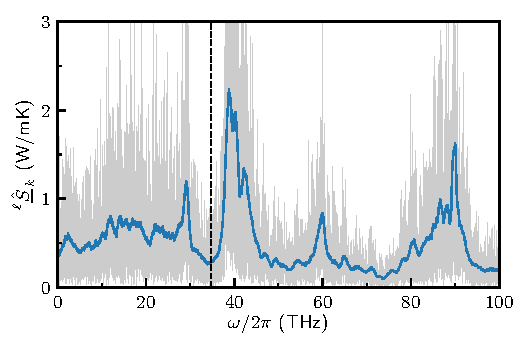
\includegraphics[width=8cm]{chapters/chapter5/figures/psd_water_ethanol_40.pdf}
\caption{Multi-component power spectrum, as defined in Eq.~\eqref{eq:mean-multi-periodogram}, for a classical flexible model of a solution of water and ethanol $50\un{mol}\%$, obtained from a $100\un{ps}$ trajectory. Grey: $^{\ell}\hat{\underline{S}}_{\,k}$ obtained directly from Eq.~\eqref{eq:mean-multi-periodogram}, with $\ell=3$ and $Q=2$. Blue: $^{\ell}\hat{\underline{S}}_{\,k}$ filtered with a moving average window of width $1\un{THz}$ in order to reveal its main features. The vertical dashed line delimits the low-frequency region used in the subsequent cepstral analysis. Reproduced from \cite{Bertossa2018}.}  \label{fig:grappa-periodogram}
\end{figure}

\begin{figure}
    \begin{center}
        \subfigure[]{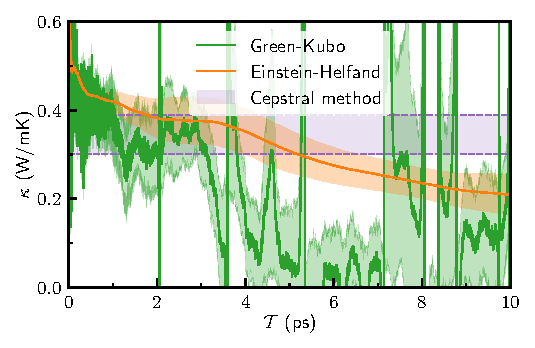
\includegraphics[width=8cm]{chapters/chapter5/figures/gk-grappa_capitolo_40.pdf}}
        \subfigure[]{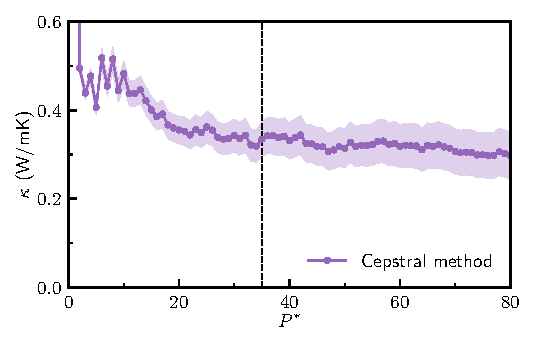
\includegraphics[width=8cm]{chapters/chapter5/figures/convergence_water_ethanol_40.pdf}}
    \end{center}
	\caption{Convergence of the multi-component thermal conductivity estimator $\kappa$ using the direct time-integration approach and the cepstral method, for a classical flexible model of a solution of water and ethanol $50\un{mol}\%$, obtained from a $100\un{ps}$ trajectory.
(a) Direct time-integration approach in its Green-Kubo (green, as obtained from the matrix $L^{ij}(\mathcal{T})\propto\int_0^\mathcal{T} \left\langle J^i(t) J^j(0) \right\rangle dt $) and Einstein-Helfand (orange -- obtained from the  matrix $\left (L^{ij}\right )'(\mathcal{T}) \propto  \int_0^\mathcal{T}\left(1-\frac{t}{\mathcal{T}}\right) \left \langle J^i(t) J^j(0) \right \rangle dt$) formulations. The horizontal purple band indicates the value obtained by the cepstral method.
(b) Estimate of $\kappa$ with the cepstral method as a function of the number of cepstral coefficients, $P^*$, see Eqs.~(\ref{eq:L0*}-\ref{eq:sigma*}). The dashed vertical line indicates the value of $P^*$ selected by the AIC, Eq.~\eqref{eq:AIC-P}. Reproduced from \cite{Bertossa2018}.
}  \label{fig:twoCompConvergence}
\end{figure}

The method discussed so far shows a fundamental advantage with respect to a na\"ive implementation of direct time-integration approach.
Fig.~\ref{fig:twoCompConvergence} shows the two-component conductivity $\kappa$, obtained via Eq.~\eqref{eq:two-comp-kappa}, in the case of a water-ethanol solution, as a function of the upper time-integration limit $\mathcal{T}$ \citep{Bertossa2018}. Both the Green-Kubo and the Einstein-Helfand definitions of the finite-time expression of Onsager's coefficients (see Eq.~\eqref{eq:Einstein-Helfand}) are displayed.
Due to thermal fluctuations, the integral of the correlation function becomes a random walk as soon as the latter vanishes, eventually assuming any value. Therefore, there will be a set of times (see Fig.~\ref{fig:twoCompConvergence}) where the term $L^{\smallQ\smallQ}$ at the denominator in Eq.~\eqref{eq:two-comp-kappa} vanishes, leading to divergences in the evaluation of $\kappa$; an issue not affecting the one-component case. Hence, in such a formulation of the multi-component case, the mean value of the thermal conductivity estimator \textit{in the time domain} does not exist. On the contrary, the multi-component frequency-domain approach presented in this section, and built on sound statistical basis, provides a well defined expression for the estimator of $\kappa$ and its statistical error.


\section{Data analysis work-flow}
We summarize the steps leading to the estimation of thermal conductivity by the \textit{cepstral analysis} method, in order to highlight the simplicity of its practical implementation.
\begin{enumerate}
\item From a MD simulation compute the heat flux time series $J_n^1$ and the independent particle fluxes $J_n^q$, $q=2,\dots,Q$.
\item Compute the discrete Fourier transform of the fluxes, $\tilde{J}^{\small i}_k$, and the element $1/(\hat{S}^{-1})^{\smallone\smallone}$. In practice, only a selected low-frequency region shall be used (see \cite{Ercole2017} for a detailed discussion).\footnote{To lighten the notation, we drop the left superscripts of the variables in this subsection.}
\item Calculate $\log\left[1/(\hat{S}^{-1})^{\smallone\smallone}\right]$.
\item Compute the inverse discrete Fourier transform of the result to obtain the cepstral coefficients $\hat{C}_n$.
\item Apply the Akaike Information Criterion, Eq.~\eqref{eq:AIC-P}, to estimate the number of cepstral coefficients to retain, $P^*$.
\item Finally apply Eq.~\eqref{eq:L0*} to obtain $\hat{L}_0^*$, and evaluate the thermal conductivity as
\begin{equation}
\kappa = \frac{\rOmega}{2k_B T^2} \exp\left[\hat{L}_0^* - \psi(\ell - Q+1) + \log(\ell -Q+1) \right],
\end{equation}
and its statistical error as
\begin{equation}
\frac{\rDelta\kappa}{\kappa} = \sqrt{\psi'(\ell -Q+1) \frac{4P^{*}-2}{N}}.
\end{equation}
\end{enumerate}
